%\documentclass{article}
\documentclass[journal,12pt,twocolumn]{IEEEtran}

% Language setting
% Replace `english' with e.g. `spanish' to change the document language
\usepackage[english]{babel}

% Set page size and margins
% Replace `letterpaper' with `a4paper' for UK/EU standard size
%%\usepackage[letterpaper,top=2cm,bottom=2cm,left=3cm,right=3cm,marginparwidth=1.75cm]{geometry}

% Useful packages
\usepackage[utf8]{inputenc}
\usepackage{enumitem}
\usepackage{multicol}
\usepackage{derivative}
\usepackage{ragged2e}
\usepackage{amsmath}
\usepackage{amssymb}
\usepackage{graphicx}
\let\vec\mathbf
\newcommand{\myvec}[1]{\ensuremath{\begin{pmatrix}#1\end{pmatrix}}}
\usepackage{array}
\usepackage{blindtext}
%\usepackage[paperwidth=10cm]{geometry}
\usepackage{tkz-euclide}
%\usepackage{tikz}
\usetikzlibrary{
  circuits.logic,
  circuits.logic.US,
  positioning
}
\usepackage[colorlinks=true, allcolors=blue]{hyperref}

\title{Optimization Assignment}
\author{Navya Valmeekam}
\begin{document}
\providecommand{\norm}[1]{\left\lVert#1\right\rVert}
\maketitle
\begin{tableofcontents}
\section{Problem}
\noindent Show that if ABC be a triangle, and P any point $PA^{2}+PB^{2}+PC^{2}$ will be a minimum when P is at the centroid. 
\\
\\
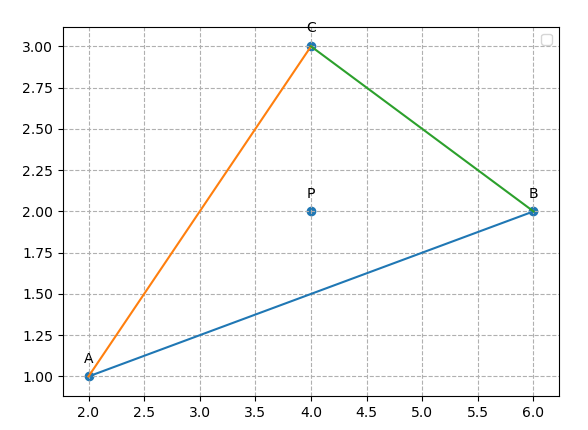
\includegraphics[scale=0.44]{opt_adv.png} 
\begin{center}
Graph
\end{center}
\vspace{0.2cm}
\section{Solution}
Let the centroid be P,
\begin{equation}
P=
\begin{pmatrix}
x\\
y
\end{pmatrix}
\end{equation}
And the function be,
\begin{equation}
f(x,y)=3x^2+3y^2-24x-12y+70
\end{equation}
\\
Using Gradient descent method,
\begin{equation}
x_n=x_{n-1}-\mu\frac{\partial f}{\partial x}
\end{equation}
\begin{equation}
\frac{\partial f}{\partial x}= 6x-24
\end{equation}
\\
\begin{equation}
y_n=y_{n-1}-\mu\frac{\partial f}{\partial y}
\end{equation}
\begin{equation}
\frac{\partial f}{\partial y}= 6y-12
\end{equation}
\\
Substituiting (4) in (3),
\begin{equation}
x_n=x_{n-1}-\mu(6x_{n-1}-24)
\end{equation} 
Substituiting (6) in (5),
\begin{equation}
y_n=y_{n-1}-\mu(6y_{n-1}-1)2
\end{equation} 
\\
Obtained values are,
\\
\vspace{3cm}
\boxed{\text{Minima Point} = 3.999,1.999 \approx 4,2}
\end{tableofcontents}
\end{document}
